%%%%%%%%%%%%%%%%%%%%%%%%%%%%%%%%%%%%%%%%%
% Beamer Presentation
% LaTeX Template
% Version 1.0 (10/11/12)
%
% This template has been downloaded from:
% http://www.LaTeXTemplates.com
%
% License:
% CC BY-NC-SA 3.0 (http://creativecommons.org/licenses/by-nc-sa/3.0/)
%
%%%%%%%%%%%%%%%%%%%%%%%%%%%%%%%%%%%%%%%%%

%----------------------------------------------------------------------------------------
%	PACKAGES AND THEMES
%----------------------------------------------------------------------------------------

\documentclass{beamer}

\mode<presentation> {

% The Beamer class comes with a number of default slide themes
% which change the colors and layouts of slides. Below this is a list
% of all the themes, uncomment each in turn to see what they look like.

%\usetheme{default}
%\usetheme{AnnArbor}
%\usetheme{Antibes}
%\usetheme{Bergen}
%\usetheme{Berkeley}
%\usetheme{Berlin}
%\usetheme{Boadilla}
%\usetheme{CambridgeUS}
%\usetheme{Copenhagen}
%\usetheme{Darmstadt}
%\usetheme{Dresden}
%\usetheme{Frankfurt}
%\usetheme{Goettingen}
%\usetheme{Hannover}
%\usetheme{Ilmenau}
%\usetheme{JuanLesPins}
%\usetheme{Luebeck}
\usetheme{Madrid}
%\usetheme{Malmoe}
%\usetheme{Marburg}
%\usetheme{Montpellier}
%\usetheme{PaloAlto}
%\usetheme{Pittsburgh}
%\usetheme{Rochester}
%\usetheme{Singapore}
%\usetheme{Szeged}
%\usetheme{Warsaw}

% As well as themes, the Beamer class has a number of color themes
% for any slide theme. Uncomment each of these in turn to see how it
% changes the colors of your current slide theme.

%\usecolortheme{albatross}
%\usecolortheme{beaver}
%\usecolortheme{beetle}
%\usecolortheme{crane}
%\usecolortheme{dolphin}
%\usecolortheme{dove}
%\usecolortheme{fly}
%\usecolortheme{lily}
%\usecolortheme{orchid}
%\usecolortheme{rose}
%\usecolortheme{seagull}
%\usecolortheme{seahorse}
%\usecolortheme{whale}
%\usecolortheme{wolverine}

%\setbeamertemplate{footline} % To remove the footer line in all slides uncomment this line
%\setbeamertemplate{footline}[page number] % To replace the footer line in all slides with a simple slide count uncomment this line

\setbeamertemplate{navigation symbols}{} % To remove the navigation symbols from the bottom of all slides uncomment this line
}

\usepackage{graphicx} % Allows including images
%\graphicspath{ {c:/Users/Eric/Documents/MHEC slides/Slides/images/} }
\usepackage{booktabs} % Allows the use of \toprule, \midrule and \bottomrule in tables

%----------------------------------------------------------------------------------------
%	TITLE PAGE
%----------------------------------------------------------------------------------------

\title[Hospital Pricing and Public Payments]{Hospital Pricing and Public Payments} % The short title appears at the bottom of every slide, the full title is only on the title page

\author[Darden, McCarthy, Barrette]{Michael Darden, Ian McCarthy, and Eric Barrette} % Your name
\institute[] % Your institution as it will appear on the bottom of every slide, may be shorthand to save space
{Midwest Health Economics Conference \\ % Your institution for the title page
\medskip
%\textit{john@smith.com} % Your email address
{Columbus, OH} 
}
\date{April 21, 2018} % Date, can be changed to a custom date

\begin{document}

\begin{frame}
\titlepage % Print the title page as the first slide
\end{frame}


%----------------------------------------------------------------------------------------
%	PRESENTATION SLIDES
%----------------------------------------------------------------------------------------

%MOTIVATION INTRO


\begin{frame}
\frametitle{Hospital Cost by Payer Type}
\begin{center}
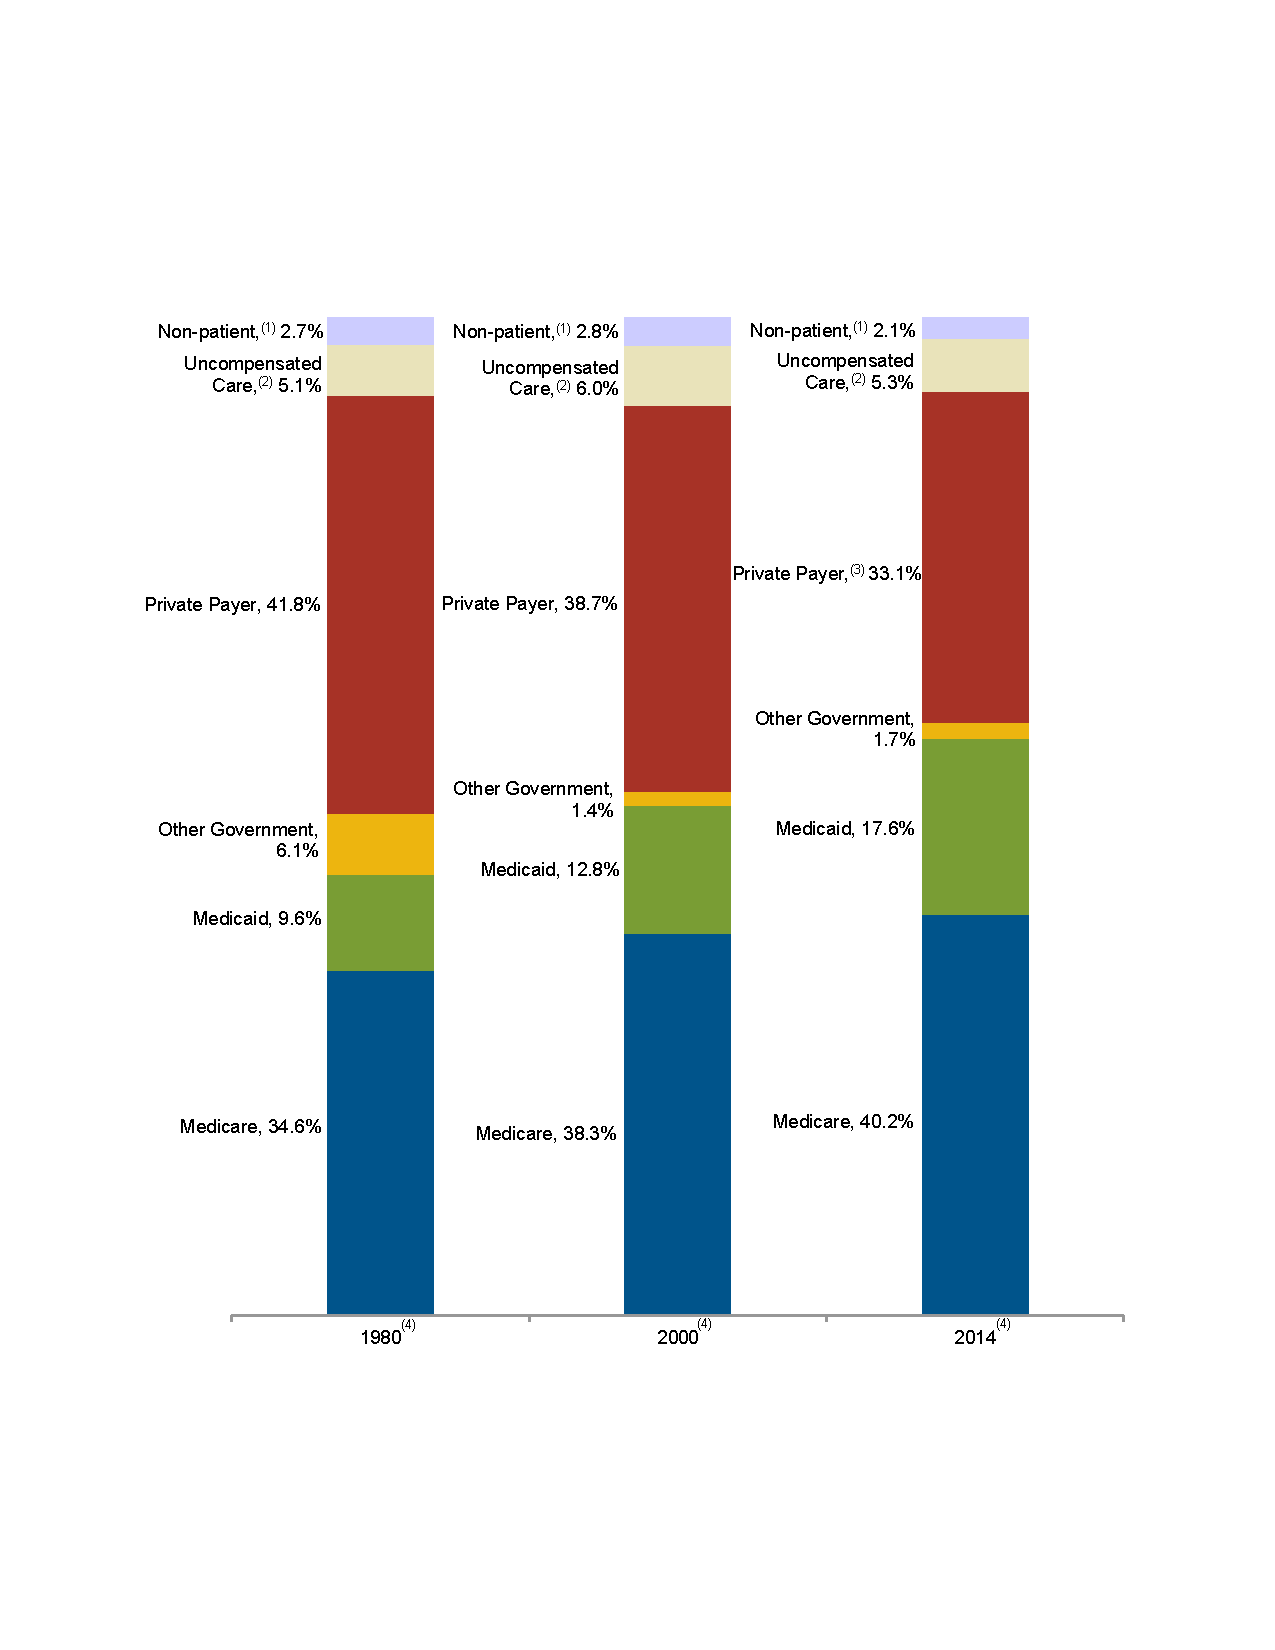
\includegraphics[scale=0.35]{4_5}
\end{center}
\tiny Source: AHA Trendwatch Chartbook 2016.  
\end{frame}

\begin{frame}
\frametitle{Payment Shortfall Relative to Costs}
\begin{center}
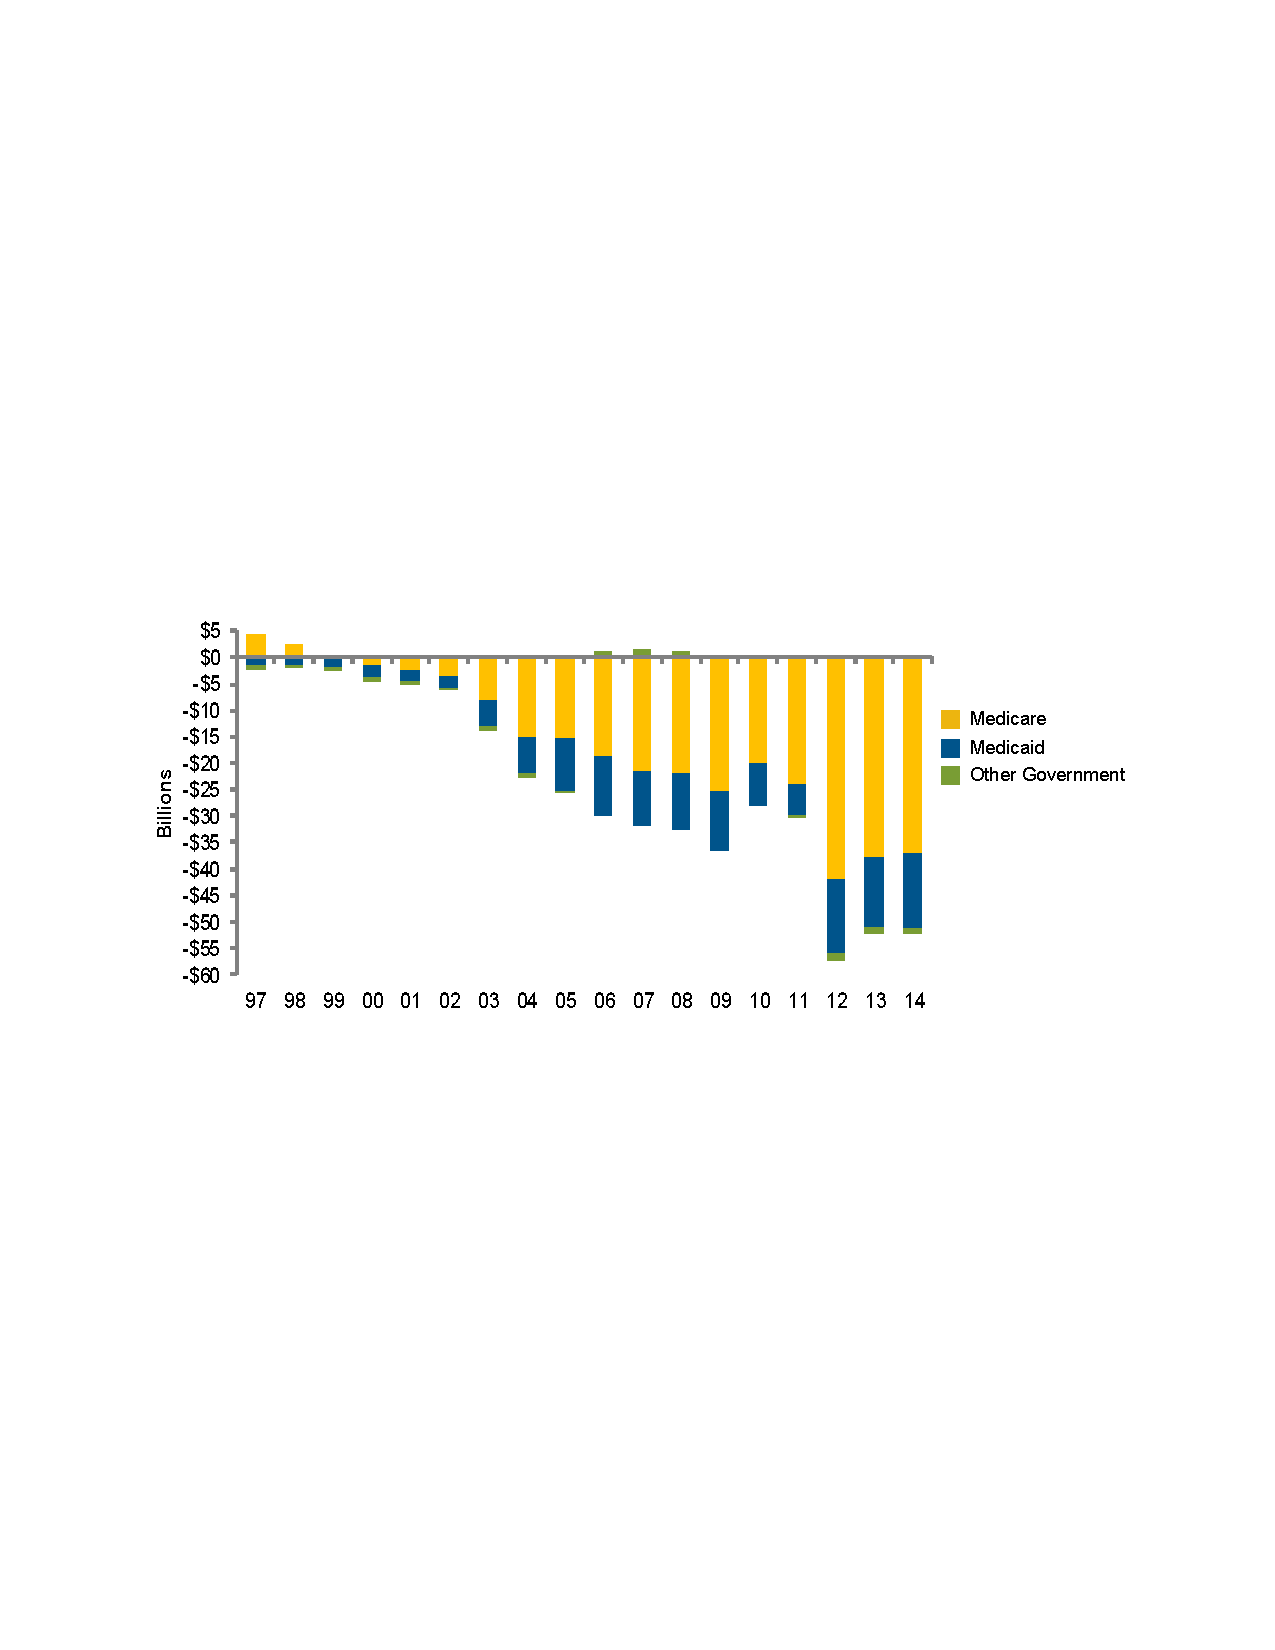
\includegraphics[scale=0.7]{4_7}
\end{center}
\tiny Source: AHA Trendwatch Chartbook 2016.  
\end{frame}

%\begin{frame}
%\frametitle{Payment-to-Cost Ratios}
%\begin{center}
%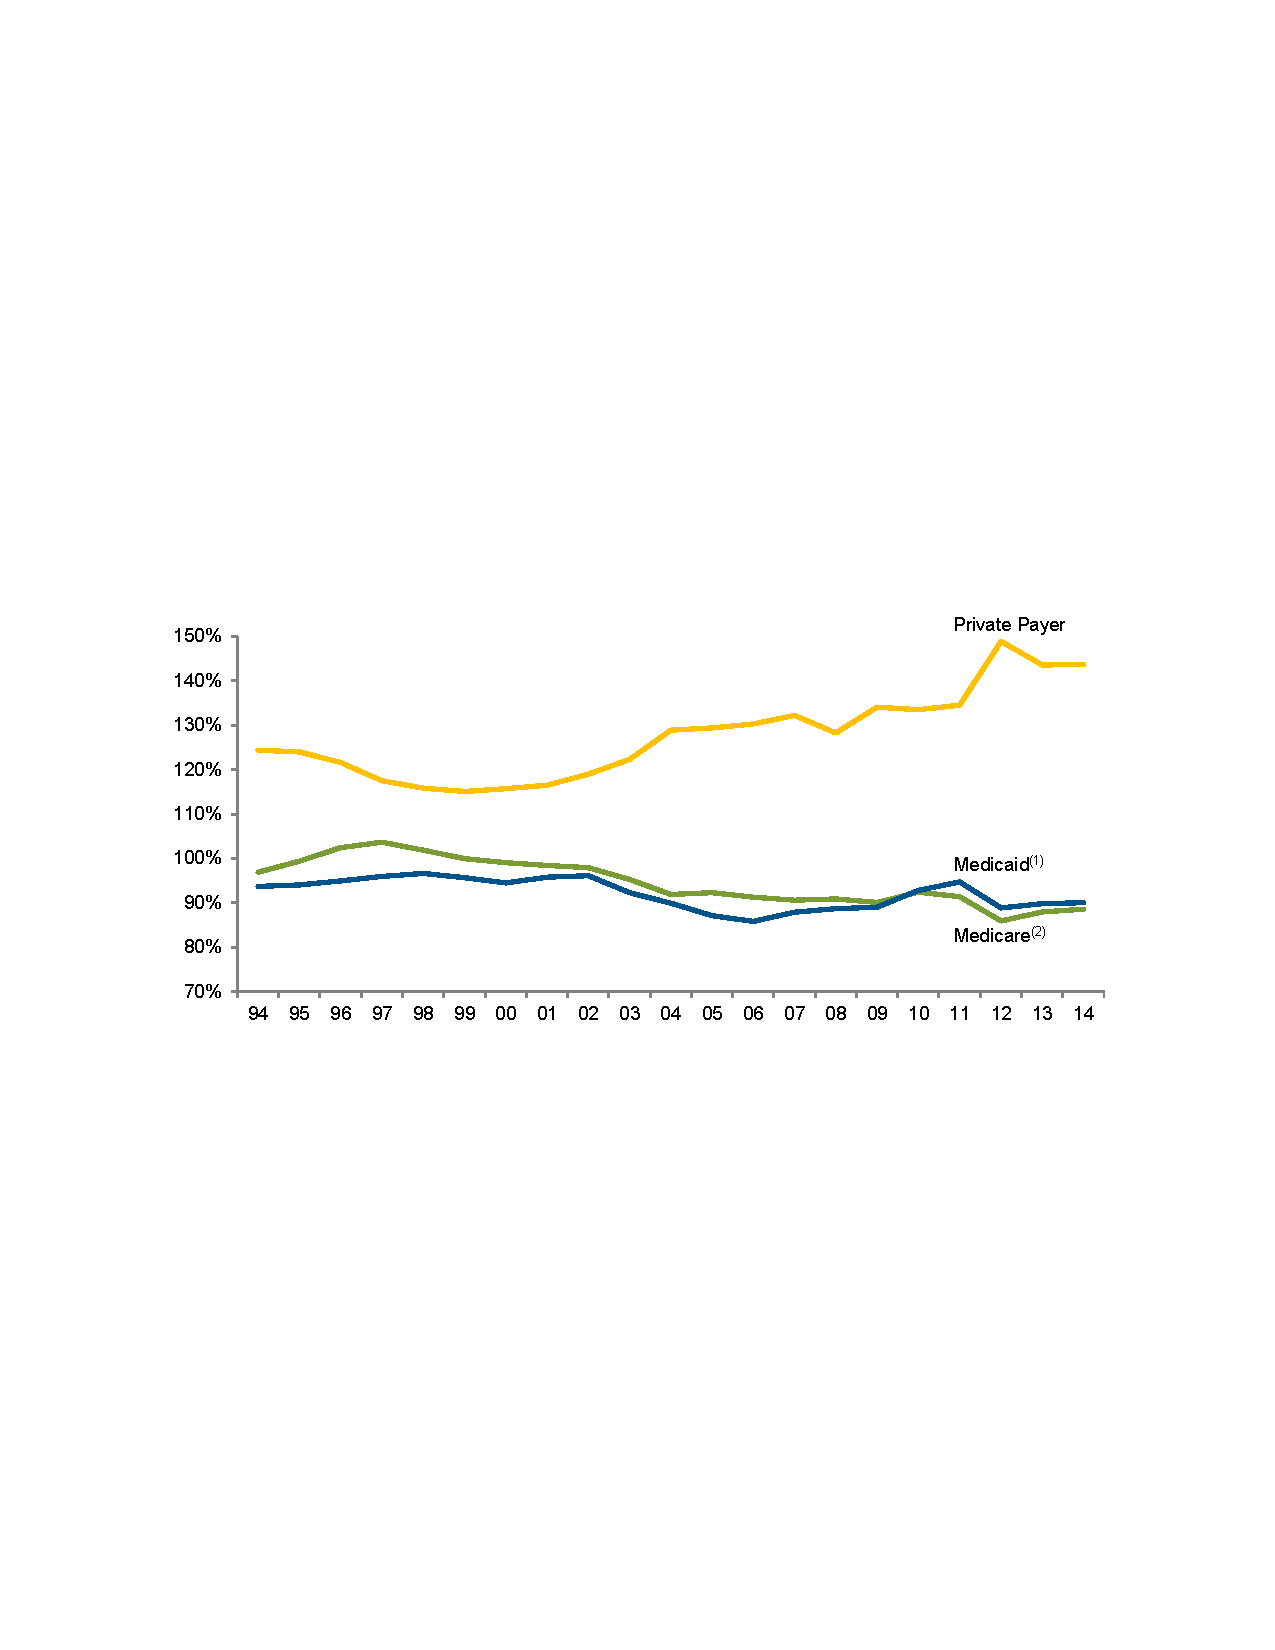
\includegraphics[scale=0.7]{4_6}
%\end{center}
%\tiny Source: AHA Trendwatch Chartbook 2016.  
%\end{frame}

\begin{frame}
\frametitle{How have hospitals responded?}
\begin{itemize}
\item ``Cost shifts have been a fact of hospital financial survival for decades.... The data show ...  how private payment is a mirror image of public payment over time and that the cost shift occurs. Hospitals must make up for shortfalls through a combination of approaches and cost-shifting is among them.'' -Rich Umbdenstock, Former President and CEO of American Hospital Association
\end{itemize}
\end{frame}

\begin{frame}
\frametitle{The ACA and Medicare?}
\begin{itemize}
\item Medicare reduced inpatient payment rates under the ACA
\item Payments were tied to quality rather than quantity through bonus payments for higher quality \textit{and} payment penalties for lower quality:
\begin{itemize}
\item Hospital Readmissions Reduction Program
\item Hospital Value-Based Purchasing Program
\item Hospital-Acquired Condition Reduction Program
\end{itemize}
\end{itemize}
\end{frame}

\begin{frame}{Research Questions}
\begin{enumerate}
\item {\bf Did hospitals respond to public reimbursement cuts by bargaining for higher prices from private insurers? (In other words... Do hospitals cost-shift?)}
\item {\bf What characteristics of hospitals are associated with cost-shifting}
\end{enumerate}
\end{frame}

\begin{frame}
\frametitle{Outline} % Table of contents slide, comment this block out to remove it
\tableofcontents % Throughout your presentation, if you choose to use \section{} and \subsection{} commands, these will automatically be printed on this slide as an overview of your presentation
\end{frame}

%------------------------------------------------
%\section{Intro} % Sections can be created in order to organize your presentation into discrete blocks, all sections and subsections are automatically printed in the table of contents as an overview of the talk
%------------------------------------------------

\section{Overview of Approach and Results}

\begin{frame}
\frametitle{Paper Overview}
\begin{itemize}
\item Approach:
\begin{itemize}
\item Plausibly exogenous variation in Medicare payments by hospital and over time due to the Hospital Readmissions Reduction Program (HRRP) and Hospital Value-Based Purchasing Program (HVBP)
\item Estimate change in commercial price using sample of ~25$\%$ of the employer-sponsored insurance population 50$\%$ of all inpatient prospective payment hospitals between 2010 and 2015
%\item[*] Papers like Cutler 1998 use changes in Medicare payment rates over time.  He notes that rates were cut almost every year in the 1980s.  Hospitals may expect cuts.  Furthermore, those cuts were the update factor not keeping up with the market basket whereas we have a discrete cut.
\end{itemize}
\item Findings:
\begin{itemize}
\item Increase in average payments of 1.0$\%$-1.4$\%$ for hospitals facing a net reimbursement reduction
\item Results consistent with effect among hospitals with better bargaining positions: %larger, statistically significant effect for hospitals with larger shares of private patients and for hospitals that were vertically integrated prior to the penalty programs.
\item Statistically significant results only for non-profit hospitals, but similar magnitude for for-profits
\item Mean effect driven by subset of admission types: circulatory and nervous system claims
\item Results not explained by changes in service mix or intensity
\end{itemize}
\end{itemize}
\end{frame}

\section{Background} 

\subsection{Cost-Shifting Literature} % A subsection can be created just before a set of slides with a common theme to further break down your presentation into chunks

\begin{frame}
\frametitle{Arguments Against Cost-Shifting} 
\begin{itemize}
\item 
Firms Shouldn't Do This:\\
``Economists usually presume that a profit-maximizing firm has previously fully exploited
all opportunities to reduce costs or raise revenues, so absent a fundamental rethinking of the firm's
strategy, it would have to absorb the loss.'' -Dranove \textit{et al.} 2017

\item Cost-shifting occurs rarley - if at all:\\
``In fact, as a whole, the evidence does not support the notion that cost-shifting is both large and
pervasive. Instead, it reveals that cost-shifting can occur but may not
always do so. When it has occurred, it has generally been measured at a
rate far below dollar-for-dollar'' - Frakt 2011
\end{itemize}
\end{frame}

\begin{frame}
\frametitle{Literature Against Cost-Shifting}
\begin{itemize}
\item Evidence Against Cost-Shifting: 
\begin{itemize}
\item Zero/Small effects: Wu (2010), Dranove (2017)
\item Lower prices: Showalter (1997), Stensland et al. (2010), White (2013)
\end{itemize}
\item Alternative Responses to Public Reimbursement Reductions
\begin{itemize}
\item Lower Profits: Garthwaite (2011)
\item Upcoding:  Dafny (2005)
\item Cutting Costs: Robinson (2011)
\item Heterogeneous Responses: Tai-Seale (1998)
\end{itemize}
\end{itemize}
\end{frame}

\begin{frame}
\frametitle{Evidence in Support of Cost-Shifting}
\begin{itemize}
\item Hospital industry claims they do it (e.g. quote from Rich Umbdenstock)
\item Insurance industry believes it happens - industry funded study found \textit{massive} cost-shifting (PWC, 2010)
\item Academic Evidence/Support for Cost-Shifting
\begin{itemize}
\item Zwanziger and Bamezai (2000, 2006)
\item Gowrisankaran and Town (1997) 
\item Clement (1998) 
\item Cutler (1998)
\end{itemize}
\end{itemize}
\end{frame}

\subsection{Medicare Payment Policy Environment}

\begin{frame}
\frametitle{Hospital Readmissions Reduction Program}
\begin{itemize}
\item Readmissions are associated with poorer outcomes and are costly:  
\begin{itemize}
%\item Concern about inpatient health.
%\item Medicare pays for readmissions except when the patient returns for treatment of the same condition within 24 h of discharge. 
\item 19.6$\%$ of all Medicare patients were readmitted within 30  
\item In 2011, Medicare's readmission rate of 17.2$\%$ resulted in 1.8 million hospitalizations within 30 days of discharge costing $\$$24bn (AHRQ 2014) 
\end{itemize}
\item HRRP reduces base payments on all Medicare inpatient admissions by a factor based on risk adjusted readmissions ratio of actual to expected based on claims lagged 2 years 
\item Penalties began in FY13 with a max reduction of 1$\%$ (increasing to 2$\%$ in FY14) based on three diagnoses: AMI, Pnuemonia, Heart Failure 
\item By FY15 the max penalty was 3$\%$ based on: AMI, Pnuemonia, Heart Failure, Hip and Knee Arthroplasty, and COPD
\end{itemize}
\end{frame}

\begin{frame}{HRRP Timeline}
\begin{table}
\centering
\footnotesize
\begin{tabular}{llll}
\hline \hline
Years penalties applied & FY 2013 & FY2014 & FY2015 \\
\hline
Diagnoses at initial hospitalization & AMI & AMI & AMI \\
						     & HF & HF & HF \\
						     & PNE & PNE & PNE \\
						     & 			&			& Hip and Knee \\
						     &			&			& COPD \\
\hline
Maximum rate of penalty		& 1$\%$ & 2$\%$ & 3$\%$ \\
Average Hospital Payment	& -0.27$\%$ & -0.25$\%$ & -0.49$\%$ \\
\hspace{0.1in} adjustment 	&&& \\
\hspace{0.1in} all hospitals	&&& \\
Average hospital penalty		& -0.42$\%$ & -0.38$\%$ & -0.63$\%$ \\
\hspace{0.1in} adjustment 	&&& \\
\hspace{0.1in} penalized hospitals	&&& \\
Percent of hospitals penalized & 64$\%$ & 66$\%$ & 78$\%$ \\
Percent of hospitals at		&8$\%$ & 0.6$\%$ & 1.2$\%$ \\
\hspace{0.1in} at max penalty	&&& \\
CMS estimate of 			& $\$$290m & $\$$227m & $\$$428m \\
\hspace{0.1in} total penalties &&&\\
\hline
\end{tabular}
\end{table}
%Emphasize the timing - lagged 3 years of data.
% Because there are no fixed quality standards and everything is relative to national mean/median, many hospitals have no incentive to change.
\end{frame}

\begin{frame}
\frametitle{Hospital Value-Based Purchasing}
%%% Principal-Agent Problem
\begin{itemize}
\item Goal is to tie 85$\%$ of fee-for-service Medicare payments to quality or value
\item All hospitals' DRG payments are reduced then penalties or bonuses based on quality: 
\begin{itemize}
\item Comparison to other hospitals
\item Comparison to their own previous performance
\end{itemize}
\item HVBP quality domains include:
\begin{itemize}
\item Clinical Process of Care: 
\item Patient Experience of Care
\item Efficiency and Cost Reduction
\item Spending
\end{itemize}
\item 2013 through 2017, payments are reduced 1$\%$, 1.25$\%$, 1.5$\%$, 1.75$\%$, and 2$\%$, respectively  
\end{itemize}
\end{frame}


\begin{frame}{HVBP Timeline}
\begin{table}
\centering
\begin{tabular}{llllll}
\hline \hline
Fiscal year   &	2013  &	2014  &	2015  &	2016	  &2017 \\
\hline
CMS withholds   &	1$\%$	  &1.25$\%$  &	1.5$\%$	  &1.75$\%$  &	2$\%$ \\
Average hospital bonus &	0.23$\%$	&	0.24$\%$	&	0.44$\%$	&	0.66$\%$	&	0.71$\%$ \\
Average hospital penalty &	0.21$\%$&		0.26$\%$	&	0.30$\%$&		0.48$\%$	&	0.48$\%$\\
Top hospital bonus &	0.83$\%$&		0.88$\%$	&	2.09$\%$&		3.02$\%$	&	4.0$\%$\\
Top hospital penalty &		0.90$\%$&		1.14$\%$	&	1.24$\%$&		1.75$\%$	&	1.83$\%$\\
\hline
\end{tabular}
\end{table}
%Above or below standard DRG reimbursement.
\tiny Source: Managed Care analysis of CMS data
\end{frame}


\begin{frame}
\frametitle{HRRP/HVBP Impacts on Quality?}
\begin{itemize}
\item Mellor \textit{et al.} (2016): HRRP associated with declines in AMI readmission, not due to delay, intensity, or patient mix
\item Gupta \textit{et al.} (2018): 5$\%$ point \textit{increase} in heart failure mortality, despite a reduction in readmissions
\item Gupta (2017): 5$\%$ reduction in overall readmissions and 3$\%$ reduction in all-cause mortality - mostly due to quality improvement
\item Desai \textit{et al.} (2016): Reduction in all readmissions following the announcement of HRRP in 2010 and a larger effect among penalized hospitals and diagnoses textit{but} impacts plateaued by start of penalties
\item Norton \textit{et al.} (2016): HVBP improved quality only for services with the highest marginal incentives to improve
\item GAO (2015): No effect of HVBP on quality - HVBP reinforced ongoing quality initiatives
\item No studies of the impact on private payer patients to our knowledge
\end{itemize}
\end{frame}


\section{Empirical Analysis}
\subsection{Identification}

\begin{frame}
\frametitle{Identification strategy}
Identification relies on the differential application of penalties across hospitals and over time (difference-in-differences)
\begin{itemize}
\item Penalties are a plausible sources of exogenous variation because
\begin{enumerate}
\item HRRP/HVBP generates variation in total hospital payments 
\item Penalties are based on lagged data that is largely beyond the hospitals control during the study period 
\end{enumerate} 
\item Use allowed payments (i.e. actual prices paid) from a national, multi-year commercial claims dataset rather than charge or cost-based measures (correlation of charge-based and allowed payments = 0.435)
\item Large sample of hospitals with a rich set of hospital-level characteristics including detailed measures of the HRRP and HVBP penalties
\end{itemize}
\end{frame}

\subsection{Data}

\begin{frame}
\frametitle{Data Sources}
\begin{itemize}
\item Commercial health insurance claims from Health Care Cost Institute
    \begin{itemize}
    \item Includes claims from 3 national commercial insurers (Aetna, UnitedHealthCare, and Humana) from all 50 states and DC. 
    \item Policies that cover 28$\%$ of Americans under 65 with employer-provided health insurance.
    \end{itemize}
\item Hospital and other regional data from:
    \begin{itemize}
    \item Hospital Compare.
    \item American Hospital Association (AHA) annual surveys
    %\item Hospital level characteristics such as bed count, system membership status, for-profit versus not-for-profit status, and teaching hospital status are from  theAmerican Hospital Association (AHA) annual surveys.
    \item Healthcare Cost Report Information System (HCRIS) 
    %\item Share of Medicare, Medicaid, and private insurance patients come from the Healthcare Cost Report Information System (HCRIS) database.
    \item American Community Survey
    \end{itemize}
    \end{itemize}
\end{frame}

\begin{frame}
\frametitle{Analytic Dataset}
Balanced panel of 1,386 inpatient prospective payment system hospitals from 2010 to 2015:
\begin{itemize}
\item Smaller hospitals and those without sufficient history (such that HRRP and HVBP don't apply) are excluded
\item Use person-level inpatient claims to calculate a hospital-level risk-adjusted average price (Gowrisankaran, Nevo, and Town (2015) Gaynor and Vogt (2003), and Cooper, et al. (2015)).: 
    \begin{itemize}
    \item Commercial price calculation uses general acute care admits within 180 miles of patient ZIP code.
    \item Excludes invalid claims and outlier payment ratios (allowed/billed) indicative of incomplete claims
    \item Regress inpatient episode payment divided by DRG weight on gender, age, and dummies for hospital in each year.
    \end{itemize}
\item Net penalty indicator accounts for possibility of HRRP penalties and HVBP penalties or bonuses
\end{itemize}
\end{frame}

\begin{frame}
\frametitle{Dependent Variables}
\begin{table}[htp]
\centering \normalsize
\caption{Characterization of Research Sample over Time}
\label{tab:samplemort}
\begin{tabular}{cccc}
\hline \hline
%\multicolumn{9}{c}{}\\
Fiscal & Sample 		&  Payment $\$$			& Percent \\
Year   &  Size    		&  Mean (St. Dev.) 			& Penalized \\
 \hline
2010 &      1,386		& 	10,729.22   (4,936.50)	& 0.00  \\
2011 &      1,386		& 	11,602.74   (5,076.45)	& 0.00   \\
2012 & 	1,386 		& 	12,079.46   (5,477.37) 	& 0.32   \\
2013 & 	1,386		& 	12,668.44   (5,567.76)	& 0.74  \\
2014 & 	1,386		&	12,795.83   (5,444.21)	& 0.76 \\
2015 &     1,386		& 	13,397.63   (5,921.74)	& 0.79 \\
&&&\\
\hline
Total & 	8,316		& 12,212.22   (5,481.55)	&	 0.43 \\
\hline
\end{tabular}
\end{table}
\end{frame}


\begin{frame}
\frametitle{Variables by Penalty Status}
\begin{table}[htp]
\centering \normalsize
\caption{Hospital Characteristics by Penalties}
\label{tab:hosp}
\begin{tabular}{lccc}
\hline \hline
Variable 	& Never 				& Ever  				& p-value  	  \\
		   		&  Penalized    		& Penalized			&       				\\
 \hline
Log(Charge) & 8.843 & 8.726 & 0.000 \\
Log(Payment) & 9.423 & 9.300 & 0.000	\\
System Membership & 0.768 & 0.784 & 0.352	\\
Non-prfit & 0.790 & 0.692 & 0.000	\\
Log(Case Mix Index) & 0.437 & 0.447 & 0.090	\\
\hline
\end{tabular}
\end{table}
\end{frame}

\subsection{Econometric Model}

\begin{frame}
\frametitle{Baseline Model}
Hospital Fixed Effects Estimator: 
\begin{equation}
\label{eq: reg}
y_{hct} = \alpha_{h} + x^{'}_{ht}\beta +  Z^{'}_{ct}\gamma+ \delta1[Penalty]  + \theta_{t}  +  \epsilon_{hct},
\end{equation}
\begin{itemize}
\item $y_{hct} =$ outcome in hospital $y$ in county $c$ in year $t$.
\item $\alpha_{h}=$ hospital fixed effect.
\item $x_{ht}=$ time-varying hospital characteristics.
\item $Z_{ct}=$ time-varying county characteristics.
\item $\theta_{t}=$ year fixed effect.
\item $\epsilon_{hct}=$ i.i.d. across hospitals and time error component.
\end{itemize}
$1[Penalty]$  penalty variable is zero in years 2010 and 2011 for all hospitals.
\end{frame}


\section{Results}
\subsection{Baseline Specification}

\begin{frame}
\frametitle{Fixed Effects Results: Baseline}
\begin{table}[htp]
\centering \normalsize
\caption{Baseline Results}
\label{tab:samplemort}
\footnotesize
\begin{tabular}{lllll1}
\hline \hline	
 			& Log Mean		& Log Mean		& Log MDCD 	   	& Log MDCR  	& Log Other  	\\
			& Payment		& Net Charge	& Discharges      		& Discharges       	& Discharges  \\
\hline
Net Penalty 	&	0.014***  & 0.008 & -0.045** & -0.027*** & -0.004	\\
	&	(0.005) & (0.008) & (0.021) & (0.007) & (0.011) 	\\
\hline
\end{tabular}
\end{table}
\tiny Notes: n = 8,316. All regressions include hospital and year fixed effects and other hospital level controls including bed count and labor force characteristics. Market power variables are constructed using the overall hospital service area. Large market is a binary variable for a hospital in the top half of the market size distribution. In cases in which independent variables are missing, we recode them and control for missing variable indicators to ensure a balanced panel. Standard errors are clustered at the hospital level. *** p-value$<$0.01, ** p-value$<$0.05, * p-value$<$0.1.
\end{frame}


\begin{frame}
\frametitle{Fixed Effects Results: Intensive Margin}
\begin{table}[htp]
\centering \normalsize
\caption{Intensive Margin Results}
\label{tab:samplemort}
\footnotesize
\begin{tabular}{llllll}
\hline \hline	
 			& Log Mean		& Log Mean		& Log MDCD 	   	& Log MDCR   		& Log Other  			\\
			& Payment		& Net Charge	& Discharges      	& Discharges       		& Discharges        	\\
\hline
Low Bonus & Omitted & & & & \\
Large 	&	-0.005 & 0.017 & 0.022 & 0.026** & 0.042**\\
\hspace{3mm}Bonus			&	(0.008) & (0.012) & (0.034) & (0.013) & (0.017)\\
Low 	&	0.010* & 0.015 & -0.026 & -0.017* & 0.004\\
\hspace{3mm}Penalty			&	(0.006) & (0.010) & (0.029) & (0.010) & (0.015)\\
Large  &	0.013* & 0.017 & -0.047 & -0.009 & 0.034**\\
\hspace{3mm}Penalty			&	(0.007) & (0.012) & (0.030) & (0.011) & (0.016)\\
\hline
\end{tabular}
\end{table}
\tiny Notes: n = 8,316. Results derived from breaking the dollar change in reimbursements above and below the median for those hospitals receiving a bonus and those receiving a penalty, respectively. All regressions include hospital and year fixed effects and other hospital level controls including bed count and labor force characteristics. Market power variables are constructed using the overall hospital service area. Large market is a binary variable for a hospital in the top half of the market size distribution. In cases in which independent variables are missing, we recode them and control for missing variable indicators to ensure a balanced panel. Standard errors are clustered at the hospital level.   *** p-value$<$0.01, ** p-value$<$0.05, * p-value$<$0.1.
\end{frame}

\begin{frame}
\frametitle{Event Study}
\begin{center}
\includegraphics[scale=0.55]{event_2panel}
\end{center}
\end{frame}

\subsection{Robustness}

\begin{frame}
\frametitle{Robustness Checks: Penalty Specific Trends}
\begin{table}[htp]
\centering \normalsize
\caption{Penalty Specific Trends Specification}
\footnotesize
\begin{tabular}{llllll}
\hline	\hline
	& Log Mean 		& Log Mean	    & Log MDCD 	   	& Log MDCR   		& Log Other  			\\
		& Payment		& Net Charge	& Discharges      & Discharges       & Discharges    \\	
\hline											
Net Penalty  	&	0.010**	&	0.018**	&	-0.037	&	-0.024***	&	-0.008	\\
	&	(0.005)	&	(0.008)	&	(0.023)	&	(0.006)	&	(0.011)	\\
p-value & 0.473 & 0.034 & 0.282 & 0.003 & 0.182 \\
\hline
\end{tabular}
\end{table}
\tiny Notes: Further controls include those in our baseline specification. The p-value is in reference to the null hypothesis that trends in the outcome of interest are the same between ever and never penalized are the same conditional on the model covariates. When independent variables are missing, we recode them and control for missing variable indicators to ensure a balanced panel. Standard errors are clustered at the hospital level. *** p-value$<$0.01, ** p-value$<$0.05, * p-value$<$0.1.
\end{frame}

\begin{frame}
\frametitle{Robustness Checks: Alternative Controls}
\begin{table}[htp]
\centering \normalsize
\caption{Net Penalty Coefficient Estimates}
\scriptsize
\begin{tabular}{llllll}
\hline	\hline
Specification	& Log Mean 		& Log Mean	  &  Log MDCD 	   	& Log MDCR   		& Log Other  \\
		& Payment		& Net Charge	& Discharges      & Discharges       & Discharges    \\	
\hline
1. Hospital, Year,  & 0.015*** & 0.009 & -0.048** & -0.027*** & -0.003 \\
\hspace{3mm}County FEs & (0.005) & (0.008) & (0.022) & (0.007) & (0.011) \\
\hline
2. Medicaid  & 0.014*** & 0.008 & -0.044** & -0.027*** & -0.005 \\
\hspace{3mm}Expansion & (0.005) & (0.008) & (0.021) & (0.007) & (0.010) \\
\hline
3. HCAHPS & 0.014*** & 0.008 & -0.045** & -0.026*** & -0.003 \\
 \hspace{3mm} Rating & (0.005) & (0.008) & (0.021) & (0.007) & (0.010) \\
\hline
4. Drop Fiscal & 0.012** & 0.010 & -0.045* & -0.028*** & -0.007 \\
 \hspace{3mm} Year 2012 & (0.005) & (0.009) & (0.023) & (0.007) & (0.012) \\
\hline
5. Case Mix & 0.014*** & 0.004 & -0.044** & -0.026*** & -0.005 \\
 \hspace{3mm} Controls & (0.005) & (0.008) & (0.021) & (0.007) & (0.011) \\
 \hline
\end{tabular}
\end{table}
\tiny Notes: Further controls include those in our baseline specification. When independent variables are missing, we recode them and control for missing variable indicators to ensure a balanced panel. Standard errors are clustered at the hospital level. *** p-value$<$0.01, ** p-value$<$0.05, * p-value$<$0.1.
\end{frame}


\subsection{Heterogeneous Effects}

\begin{frame}
\frametitle{Modeling Heterogeneous Effects}
\begin{itemize}
\item Dranove (1988) finds hospitals may cost-shift if their objective functions includes something other than pure profit (e.g. quantity) which suggests cost-shifting is more likely among non-profit hospitals.
\item We examine the conditions necessary for cost-shifting by embedding the Dranove (1988) model in a hospital-insurer bargaining model (e.g. Ho and Lee, 2017 or Gowrisankaran et al., 2015).
\item Hospitals must have some diminishing marginal utility of profits for cost-shifting to occur but do not need to derive utility from something other than profits.
\end{itemize}
\end{frame}

\begin{frame}
\frametitle{Theoretical Predictions of Heterogeneous Effects}
\begin{itemize}
\item Assuming diminishing marginal utility reflects risk-aversion (e.g., uncertain demand or uncertain “exposure” to the HVBP/HRRP penalties), our model predicts:
\begin{enumerate}
\item Any risk-averse hospital to potentially cost shift, regardless of whether the hospital is for-profit or non-profit. 
\item Cost-shifting should be largest for hospitals with more bargaining power or a better bargaining position.
\end{enumerate}
\end{itemize}
\end{frame}

\begin{frame}
\frametitle{Heterogeneity by Objective Function}
\begin{table}[htp]
\centering \normalsize
\caption{Net Penalty Coefficient Estimates by Profit Status}
\scriptsize
\begin{tabular}{llllll}
\hline	\hline
Baseline Model	& Log Mean 		& Log Mean	   & Log MDCD 	   	& Log MDCR   		& Other  			\\
		& Payment		& Net Charge	& Discharges      & Discharges       & Discharges    \\	
\hline
Non-profit & 0.015*** & 0.008 & -0.046* & -0.029*** & -0.011  \\
 & (0.005) & (0.009) & (0.024) & (0.007) & (0.012)  \\
\hline
For-profit:  & 0.020 & 0.023 & -0.018 & -0.008 & 0.026 \\
 & (0.014) & (0.021) & (0.050) & (0.018) & (0.020)  \\
\hline \hline
Penalty Specific & & & & & \\
Trends & & & & & \\
\hline
Non-profit & 0.012** & 0.015* & -0.039 & -0.023*** & -0.015  \\
 & (0.005) & (0.009) & (0.026) & (0.007) & (0.014)  \\
p-value & 0.805 & 0.205 & 0.241 & 0.001 & 0.849  \\
\hline
For-profit:  & 0.011 & 0.043* & 0.002 & -0.028 & 0.007  \\
 & (0.014) & (0.023) & (0.050) & (0.017) & (0.020)  \\
 p-value & 0.417 & 0.025 & 0.885 & 0.013 & 0.003  \\
\hline 
\end{tabular}
\end{table}
\tiny Notes: Further controls include those in our baseline specification. The p-value is in reference to the null hypothesis that trends in the outcome of interest are the same between ever and never penalized are the same conditional on the model covariates. When independent variables are missing, we recode them and control for missing variable indicators to ensure a balanced panel. Standard errors are clustered at the hospital level. *** p-value$<$0.01, ** p-value$<$0.05, * p-value$<$0.1.
\end{frame}

\begin{frame}
\frametitle{Heterogeneity by Bargaining Position}
\begin{table}[htp]
\centering \normalsize
\caption{Triple Difference by Payer Mix}
\scriptsize
\begin{tabular}{lll}
\hline	
 		& Log Mean & Log Mean   				 \\
		& Payment & Charge\\
\hline \hline
Net Penalty	& 0.039*** & 0.043*** 	\\
	&	(0.010) & (0.013)	\\
\hspace{0.1in}* Public Share 2 & -0.020* & -0.014	\\
	&	(0.012) & (0.014) 	\\
\hspace{0.1in}* Public Share 3 & -0.033** & -0.043***	\\
	&	(0.013) & (0.015) 	\\
\hspace{0.1in}* Public Share 4 & -0.044*** & -0.070***	\\
	&	(0.013) & (0.016)	\\
Public Share 2 & 0.007 & 0.049***	\\
	&	(0.010) & (0.013)	\\
Public Share 3 & 0.016 & 0.087***	\\
	&	(0.011) & (0.016) 	\\
Public Share 4 & 0.023* & 0.157***	\\
	&	(0.012) & (0.018)	\\
\hline
\end{tabular}
\end{table}
\tiny Notes: All regressions include hospital and year fixed effects. Further controls include those in our baseline specification for mean payments. The share of a hospital’s patients insured by the public sector is broken into quartiles and interacted with penalty variables. In cases in which independent variables are missing, we recode them and control for missing variable indicators to ensure a balanced panel. Standard errors are clustered at the hospital level. *** p-value$<$0.01, ** p-value$<$0.05, * p-value$<$0.1.
\end{frame}

\begin{frame}
\frametitle{Heterogeneity by Vertical Integration}
\begin{table}[htp]
\centering \normalsize
\caption{Net Penalty Coefficient Estimates by VI Status}
\footnotesize
\begin{tabular}{llllll}
\hline	\hline
 			& Log Mean 		& Log Mean	& Log MDCD 	   	& Log MDCR   		& Other  			\\
			& Payment		& 	Charge	& Discharges      	& Discharges       	& Discharges    \\
\hline											
VI prior 	&	0.023*** & 0.017*** & -0.036 & -0.026** & 0.008 	\\
\hspace{3mm}to 2012			&	(0.008) & (0.006) & (0.032) & (0.009) & (0.016) 	\\
\hline											
Never VI 	&	0.008 & 0.021*** &  -0.063** &  -0.024** &  -0.005 	\\
			&	(0.007) & (0.012) & (0.031) & (0.010) & (0.015) 	\\
\hline
\end{tabular}
\end{table}
\tiny Notes: Further controls include those in our baseline specification for mean payments. In cases in which independent variables are missing, we recode them and control for missing variable indicators to ensure a balanced panel. Standard errors are clustered at the hospital level. *** p-value$<$0.01, ** p-value$<$0.05, * p-value$<$0.1.
\end{frame}

\begin{frame}
\frametitle{Heterogeneity by Service Line}
\begin{table}[htp]
\centering \normalsize
\caption{Condition Specific Admissions}
\scriptsize
\begin{tabular}{lll1}
\hline	
 		& n & Mean & Net Penalty \\
		& & Payment & Coefficient \\
\hline \hline
Nervous	System & 1,410 & 13,762.86 & 0.021*** \\
& & & (0.010)\\
Respiratory System & 1,758 & 12,015.13 & 0.001 \\
& & &  (0.011)\\
Circulatory System & 2,754 & 13,071.17 & 0.019** \\
& & &  (0.008)\\
Musculoskeletal System & 3,060 & 12,981.58 & 0.004\\
& & &  (0.007)\\
Labor and Delivery & 5,226 & 11,308.56 & -0.001 \\
& & &  (0.005) \\
Neonatal & 3,204 & 8,911.19  & 0.016 \\
& & &  (0.010) \\
\hline
\end{tabular}
\end{table}
\tiny Notes: We restrict the sample to include at least 25 admissions per hospital per year. The dependent variable is the log of average payments for each associated acute care admission category. The net penalty coefficient is estimated from the baseline specification.  Standard errors are clustered at the hospital level.   *** p-value$<$0.01, ** p-value$<$0.05, * p-value$<$0.1.
\end{frame}



\section{Discussion of Potential Alternative Explanations}

\begin{frame}
\frametitle{Potential Alternative Explanations}
\begin{itemize}
\item 
Did hospitals improve quality that private insurers are willing to pay more for? 
 \begin{itemize}
 \item
 Mixed evidence of quality improvements and unclear if private payer patients quality improved following HRRP/HVBP
 \end{itemize}
\item
Are hospitals are changing the service mix?
 \begin{itemize}
 \item
No evidence of more profitable services?  
 \item
No evidence of higher intensity of services?
 \end{itemize}
\end{itemize}
\begin{table}[htp]
\centering \normalsize
\caption{Test of Changes in Service Use}
\begin{tabular}{c|ccc}
\hline
& Profit Index & Mean DRG Weight & Mean LOS \\
\hline \hline
Net Penalty & 0.002 & 0.004 & 0.015  \\
 & (0.001) & (0.004) & (0.012)  \\
\hline
\end{tabular}
\end{table}
\tiny Notes: n = 8,316. The net penalty coefficient is estimated from the baseline specification. Standard errors are clustered at the hospital level.   *** p-value$<$0.01, ** p-value$<$0.05, * p-value$<$0.1.

\end{frame}




\section{Conclusion}

\begin{frame}
\frametitle{Conclusion}
\begin{itemize}
\item 
Baseline estimate of 1.4$\%$ increase in commercial prices for hospitals that were penalized under the HRRP/HVBP programs.
\begin{itemize}
\item 
Result is robust to a variety of alternative specifications - no evidence of changes in underlying quality or intensity of treatment. 
\item 
Estimate implies an increase of $\$$167 per inpatient stay based on an average private insurance payment of approximately $\$$12,100 among penalized hospitals
\item
Accounting for differential trends with hospital fixed effects controlling for time-varying unobserved heterogeneity, the estimated effect is still significant: 1$\%$ 
\end{itemize}
\item
These results should not be interpreted as pay for performance is inherently bad rather that the design of the pay for performance program is important 
\end{itemize}
\end{frame}

\end{document}